\documentclass[a4paper,11pt,twoside]{article}
\usepackage[utf8]{inputenc}
\usepackage[T1]{fontenc}
\usepackage{boldline,multirow,tabularx,colortbl}
\usepackage{amsfonts,amssymb,amsmath,mathrsfs}
\usepackage{pgf,tikz,xcolor}
\usetikzlibrary{calc,positioning,shapes.geometric,shapes.symbols,shapes.misc, fit, shapes, arrows}
\usepackage[top=2cm, bottom=2cm, left=2cm, right=2cm]{geometry}
\usepackage{hyperref}
\usepackage{titlesec}
\usepackage[titles]{tocloft}
\usepackage[francais]{babel}

\tikzset{
    circlenode/.style={ % requires library shapes.misc
        draw,
        circle,
        align=center,
        fill=gray!5!white
    }
}
\newcommand\tab[1][0.6cm]{\hspace*{#1}} %Create and define tab

\definecolor{lightgray}{gray}{0.75}

\addtolength{\cftsecnumwidth}{12pt} %Spacing correction in table of contents


%------- Do not append new commands after :

\hypersetup{	
    colorlinks=false, % colorise les liens
    linkbordercolor={1 1 1},
    breaklinks=true, % permet le retour à la ligne dans les liens trop longs
    urlcolor=blue, % couleur des hyperliens 
    linkcolor=black,	% couleur des liens internes 
    citecolor=black,	% couleur des références 
    pdftitle={Problèmes du Projet Euler - Traduction Française}, % informations apparaissant dans 
    pdfauthor={Rémi Gascou}, % les informations du document 
    pdfsubject={}	% sous Acrobat. 
}

%Main Title
\def\maintitle{Project Euler Problems}

%Main Subtitle (useful to for indicating in which language it is translated)
\def\mainsubtitle{Original Version}

%Name of the Translator
\def\translatorname{Rémi GASCOU}

%Header of the Table of contents
\def\tocheader{Problems Summary}

%Word appearing before numbering and section name.
\def\beforesectionnumbering{Problem}

\titleformat{\section}{\normalfont\large\bfseries}{\beforesectionnumbering\text{ }\thesection  - }{0em}{}

\title{\vspace{7cm}\Huge{\maintitle} \\ \vspace{1cm} \LARGE{\mainsubtitle}\vspace{3cm}}
\author{}
\date{}


\begin{document}
    \renewcommand{\contentsname}{\begin{center}\tocheader \end{center}}
    \maketitle
    \pagenumbering{gobble}
    \newpage
    
    \begin{center}
         
        \vspace{11cm}
        
        Translated by \translatorname\\
        \bigskip
        $-$ Version of \today $-$ 
    \end{center}
    
    \newpage \newpage
    
    \pagenumbering{arabic}
    \setcounter{page}{1}
    \tableofcontents
    
    \section*{Préface} \addcontentsline{toc}{section}{Préface}

\begin{center}
    %\LARGE{\textit{"Project Euler exists to encourage, challenge, and develop the skills and enjoyment of anyone with an interest in the fascinating world of mathematics."}}
    
    \LARGE{\textit{"Le Projet Euler est là pour encourager, stimuler, et développer les compétences de chacun portant son intérêt au monde fascinant des mathématiques."}}
    
\end{center}

Lorem ipsum dolor sit amet, consectetur adipiscing elit. Mauris hendrerit ut odio sed luctus. Aliquam sit amet lobortis sem, nec faucibus tellus. Donec nulla nunc, porttitor quis dolor in, maximus rutrum tortor. Donec fringilla hendrerit lorem viverra efficitur. Etiam at mi ante. Aliquam quis elementum arcu. Suspendisse commodo dui eget ex ornare convallis ac id mauris. Phasellus non convallis purus. Maecenas euismod tellus eu lectus vehicula blandit. Integer gravida lacinia tincidunt. Integer et turpis ante. Maecenas libero felis, condimentum sed scelerisque a, feugiat in enim.


Phasellus bibendum, ante eu tincidunt pretium, mi felis dignissim magna, nec scelerisque velit justo sit amet urna. Curabitur gravida mi ex, non consequat urna efficitur sed. Cras ac euismod lectus. Nulla non tortor pharetra velit posuere semper semper eget diam. Integer lobortis purus at sapien viverra, ut aliquet dui pellentesque. Aliquam molestie lorem in erat iaculis mollis. Morbi sodales accumsan est eget sagittis. Fusce vel.



\begin{flushright}
    \textit{{Rémi Gascou}}
\end{flushright}

\vspace{5cm}

\begin{center}
    Tous les problèmes sont tirés du site :
    
    \href{https://projecteuler.net/}{https://projecteuler.net/}
\end{center}
    %\setcounter{section}{24}
    %\part*{\begin{center}Les problèmes (1 à 600)\end{center}}
    %\include{problems_FR/1-100/pack_0001-0100}
    \setcounter{section}{100}
\section{Optimum polynomial} \label{pb.0101}
%PB101

If we are presented with the first $k$ terms of a sequence it is impossible to say with certainty the value of the next term, as there are infinitely many polynomial functions that can model the sequence.

As an example, let us consider the sequence of cube numbers. This is defined by the generating function,
$$u_n = n^3: 1, 8, 27, 64, 125, 216, ...$$

Suppose we were only given the first two terms of this sequence. Working on the principle that "simple is best" we should assume a linear relationship and predict the next term to be 15 (common difference 7). Even if we were presented with the first three terms, by the same principle of simplicity, a quadratic relationship should be assumed.

We shall define $OP(k, n)$ to be the $n^{\text{th}}$ term of the optimum polynomial generating function for the first $k$ terms of a sequence. It should be clear that $OP(k, n)$ will accurately generate the terms of the sequence for $n \leqslant k$, and potentially the first incorrect term (FIT) will be $OP(k, k+1)$; in which case we shall call it a bad OP (BOP).

As a basis, if we were only given the first term of sequence, it would be most sensible to assume constancy; that is, for $n \geqslant 2$, $OP(1, n) = u_1$.

Hence we obtain the following OPs for the cubic sequence:


\begin{center}
    \begin{tabular}{ll}
        $OP(1, n) = 1$ & 1, \textcolor[rgb]{1,0,0}{1}, 1, 1, ...\\
        $OP(2, n) = 7n-6$ & 1, 8, \textcolor[rgb]{1,0,0}{15}, ...\\
        $OP(3, n) = 6n^2-11n+6$ & 1, 8, 27, \textcolor[rgb]{1,0,0}{58}, ...\\
        $OP(4, n) = n^3$ & 1, 8, 27, 64, 125, ...\\
    \end{tabular}
\end{center}

Clearly no BOPs exist for $k \geqslant 4$.

By considering the sum of FITs generated by the BOPs (indicated in \textcolor[rgb]{1,0,0}{red} above), we obtain:
$$1 + 15 + 58 = 74$$

Consider the following tenth degree polynomial generating function:

$$u_n = 1 - n + n^2 - n^3 + n^4 - n^5 + n^6 - n^7 + n^8 - n^9 + n^{10}$$

Find the sum of FITs for the BOPs.


\section{Triangle containment} \label{pb.0102}
%PB102

Three distinct points are plotted at random on a Cartesian plane, for which $-1000 \leqslant x, y \leqslant 1000$, such that a triangle is formed.

Consider the following two triangles:

$$A(-340,495), B(-153,-910), C(835,-947)$$
$$X(-175,41), Y(-421,-714), Z(574,-645)$$

It can be verified that triangle $ABC$ contains the origin, whereas triangle $XYZ$ does not.
\smallskip

Using \href{https://projecteuler.net/project/resources/p102_triangles.txt}{triangles.txt} (right click and 'Save Link/Target As...'), a 27K text file containing the co-ordinates of one thousand "random" triangles, find the number of triangles for which the interior contains the origin.
\smallskip

\textbf{NOTE:} The first two examples in the file represent the triangles in the example given above.

\newpage


\section{Special subset sums: optimum} \label{pb.0103}
%PB103

Let $S(A)$ represent the sum of elements in set $A$ of size $n$. We shall call it a special sum set if for any two non-empty disjoint subsets, $B$ and $C$, the following properties are true:
\medskip

\begin{itemize}
    \item $S(B) \neq S(C)$; that is, sums of subsets cannot be equal.
    \item If $B$ contains more elements than $C$ then $S(B) > S(C)$.
\end{itemize}
\medskip

If $S(A)$ is minimised for a given $n$, we shall call it an optimum special sum set. The first five optimum special sum sets are given below.

\begin{center}
    \begin{tabular}{cl}
        $n = 1$ & {1}\\
        $n = 2$ & {1, 2}\\
        $n = 3$ & {2, 3, 4}\\
        $n = 4$ & {3, 5, 6, 7}\\
        $n = 5$ & {6, 9, 11, 12, 13}\\
    \end{tabular}
\end{center}

It seems that for a given optimum set, $A = {a_1, a_2, ... , a_n}$, the next optimum set is of the form $B = {b, a_1+b, a_2+b, ... ,a_n+b}$, where $b$ is the "middle" element on the previous row.
\medskip

By applying this "rule" we would expect the optimum set for $n = 6$ to be $A = {11, 17, 20, 22, 23, 24}$, with $S(A) = 117$. However, this is not the optimum set, as we have merely applied an algorithm to provide a near optimum set. The optimum set for $n = 6$ is $A = {11, 18, 19, 20, 22, 25}$, with $S(A) = 115$ and corresponding set string: 111819202225.
\medskip

Given that $A$ is an optimum special sum set for $n = 7$, find its set string.
\medskip

\textbf{NOTE:} This problem is related to \hyperref[pb.0105]{\textbf{Problem 105}} and \hyperref[pb.0106]{\textbf{Problem 106}}.


\section{Pandigital Fibonacci ends} \label{pb.0104}
%PB104

The Fibonacci sequence is defined by the recurrence relation:

$$F_n = F_{n-1} + F_{n-2}, \text{ where } F_1 = 1 \text{ and } F_2 = 1$$

It turns out that $F_{541}$, which contains 113 digits, is the first Fibonacci number for which the last nine digits are 1-9 pandigital (contain all the digits 1 to 9, but not necessarily in order). And $F_{2749}$, which contains 575 digits, is the first Fibonacci number for which the first nine digits are 1-9 pandigital.
\medskip

Given that $F_k$ is the first Fibonacci number for which the first nine digits AND the last nine digits are 1-9 pandigital, find $k$.

\newpage


\section{Special subset sums: testing} \label{pb.0105}
%PB105

Let $S(A)$ represent the sum of elements in set $A$ of size $n$. We shall call it a special sum set if for any two non-empty disjoint subsets, $B$ and $C$, the following properties are true:
\medskip

\begin{itemize}
    \item $S(B) \neq S(C)$; that is, sums of subsets cannot be equal.
    \item If $B$ contains more elements than $C$ then $S(B) > S(C)$.
\end{itemize}
\medskip

For example, ${81, 88, 75, 42, 87, 84, 86, 65}$ is not a special sum set because 65 + 87 + 88 = 75 + 81 + 84, whereas ${157, 150, 164, 119, 79, 159, 161, 139, 158}$ satisfies both rules for all possible subset pair combinations and $S(A) = 1286$.

Using \href{https://projecteuler.net/project/resources/p105_sets.txt}{sets.txt} (right click and "Save Link/Target As..."), a 4K text file with one-hundred sets containing seven to twelve elements (the two examples given above are the first two sets in the file), identify all the special sum sets, $A_1, A_2, ..., A_k$, and find the value of $S(A_1) + S(A_2) + ... + S(A_k)$.

\textbf{NOTE:} This problem is related to \hyperref[pb.0103]{\textbf{Problem 103}} and \hyperref[pb.0106]{\textbf{Problem 106}}.


\section{Special subset sums: meta-testing} \label{pb.0106}
%PB106

Let $S(A)$ represent the sum of elements in set $A$ of size $n$. We shall call it a special sum set if for any two non-empty disjoint subsets, $B$ and $C$, the following properties are true:
\medskip

\begin{itemize}
    \item $S(B) \neq S(C)$; that is, sums of subsets cannot be equal.
    \item If $B$ contains more elements than $C$ then $S(B) > S(C)$.
\end{itemize}
\medskip

For this problem we shall assume that a given set contains $n$ strictly increasing elements and it already satisfies the second rule.

Surprisingly, out of the 25 possible subset pairs that can be obtained from a set for which $n = 4$, only 1 of these pairs need to be tested for equality (first rule). Similarly, when $n = 7$, only 70 out of the 966 subset pairs need to be tested.

For $n = 12$, how many of the 261625 subset pairs that can be obtained need to be tested for equality?

\textbf{NOTE:} This problem is related to \hyperref[pb.0103]{\textbf{Problem 103}} and \hyperref[pb.0105]{\textbf{Problem 105}}.

\newpage


\section{Minimal network} \label{pb.0107}
%PB107

The following undirected network consists of seven vertices and twelve edges with a total weight of 243.

%tikz

\begin{center}
    \begin{tikzpicture}
        \def\len{75}
        \node[below] (D) {D};
        \node[above left = \len pt and 0.6*\len pt of D] (B) {B};
        \node[above right = \len pt and 0.6*\len pt of D] (E) {E};
        \node[right = 1.35*\len pt of D] (G) {G};
        \node[below left = \len pt and 0.6*\len pt of D] (C) {C};
        \node[below right = \len pt and 0.6*\len pt of D] (F) {F};
        \node[left = 1.35*\len pt of D] (A) {A};
        
        \draw (A) -- (D) -- (G);
        \draw (B) -- (D) -- (F);
        \draw (C) -- (D) -- (E);
        \draw (B) -- (E) -- (G) -- (F) -- (C) -- (A) -- (B);
        
        \node[above left = \len/2 pt and 0.6*\len/2 pt of D,circlenode] (midDB) {17};
        \node[above right = \len/2 pt and 0.6*\len/2 pt of D,circlenode] (midDE) {18};
        \node[right = 1.35*\len/2 pt of D,circlenode] (midDG) {23};
        \node[below right = \len/2 pt and 0.6*\len/2 pt of D,circlenode] (midDF) {19};
        \node[below left = \len/2 pt and 0.6*\len/2 pt of D,circlenode] (midDC) {28};
        \node[left = 1.35*\len/2 pt of D,circlenode] (midDA) {21};
        
        \node[above = \len-5 pt of D,circlenode] (midBE) {20};
        \node[below = \len-5 pt of D,circlenode] (midCF) {31};
    \end{tikzpicture}
\end{center}

The same network can be represented by the matrix below.

\begin{center}
    \begin{tabular}{|l|*{8}{c|}}
        \hline
        \rowcolor{lightgray} & A & B & C & D & E & F & G\\
        \hline
        \cellcolor{lightgray}{A} & - & 16 & 12 & 21 & - & - & -\\
        \hline
        \cellcolor{lightgray}{B} & 16 & - & - & 17 & 20 & - & -\\
        \hline
        \cellcolor{lightgray}{C} & 12 & - & - & 28 & - & 31 & -\\
        \hline
        \cellcolor{lightgray}{D} & 21 & 17 & 28 & - & 18 & 19 & 23\\
        \hline
        \cellcolor{lightgray}{E} & - & 20 & - & 18 & - & - & 11\\
        \hline
        \cellcolor{lightgray}{F} & - & - & 31 & 19 & - & - & 27\\
        \hline
        \cellcolor{lightgray}{G} & - & - & - & 23 & 11 & 27 & -\\
        \hline
    \end{tabular}
\end{center}


However, it is possible to optimise the network by removing some edges and still ensure that all points on the network remain connected. The network which achieves the maximum saving is shown below. It has a weight of 93, representing a saving of $243 - 93 = 150$ from the original network.

\begin{center}
    \begin{tikzpicture}
        \def\len{75}
        \node[below] (D) {D};
        \node[above left = \len pt and 0.5*\len pt of D] (B) {B};
        \node[above right = \len pt and 0.5*\len pt of D] (E) {E};
        \node[right = 1.35*\len pt of D] (G) {G};
        \node[below left = \len pt and 0.5*\len pt of D] (C) {C};
        \node[below right = \len pt and 0.5*\len pt of D] (F) {F};
        \node[left = 1.35*\len pt of D] (A) {A};
        
        
        \draw (C) -- (A) -- (B) -- (D) -- (F);
        \draw (D) -- (E) -- (G);
        
        
        \node[above left = \len/2 pt and 0.5*\len/2 pt of D,circlenode] (midDB) {17};
        \node[above right = \len/2 pt and 0.5*\len/2 pt of D,circlenode] (midDE) {18};
        \node[below right = \len/2 pt and 0.5*\len/2 pt of D,circlenode] (midDF) {19};

        
    \end{tikzpicture}
\end{center}

Using \href{https://projecteuler.net/project/resources/p107_network.txt}{\textbf{network.txt}} (right click and 'Save Link/Target As...'), a 6K text file containing a network with forty vertices, and given in matrix form, find the maximum saving which can be achieved by removing redundant edges whilst ensuring that the network remains connected.


\newpage


\section{Diophantine reciprocals I} \label{pb.0108}
%PB108

In the following equation $x, y$, and $n$ are positive integers.

$$\frac{1}{x} + \frac{1}{y} = \frac{1}{n}$$

For $n = 4$ there are exactly three distinct solutions:

$$\frac{1}{5} + \frac{1}{20} = \frac{1}{4}$$
$$\frac{1}{6} + \frac{1}{12} = \frac{1}{4}$$
$$\frac{1}{8} + \frac{1}{8} = \frac{1}{4}$$

What is the least value of $n$ for which the number of distinct solutions exceeds one-thousand?
\medskip

\textbf{NOTE:} This problem is an easier version of \hyperref[pb.0110]{\textbf{Problem 110}}; it is strongly advised that you solve this one first.


\section{Darts} \label{pb.0109}
%PB109

In the game of darts a player throws three darts at a target board which is split into twenty equal sized sections numbered one to twenty.


\begin{center}
    \begin{tikzpicture}
        \node[anchor=south west,inner sep=0] at (0,0) {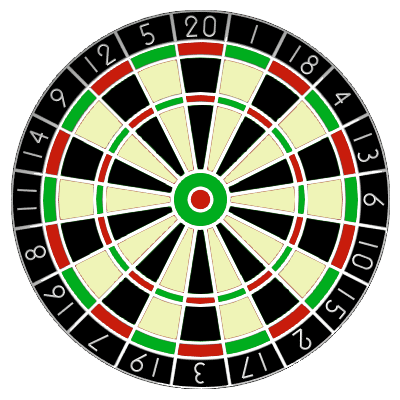
\includegraphics[width=70mm]{problems/101-200/meta/p109.png}};
    \end{tikzpicture}
\end{center}

The score of a dart is determined by the number of the region that the dart lands in. A dart landing outside the red/green outer ring scores zero. The black and cream regions inside this ring represent single scores. However, the red/green outer ring and middle ring score double and treble scores respectively.

At the centre of the board are two concentric circles called the bull region, or bulls-eye. The outer bull is worth 25 points and the inner bull is a double, worth 50 points.

There are many variations of rules but in the most popular game the players will begin with a score 301 or 501 and the first player to reduce their running total to zero is a winner. However, it is normal to play a "doubles out" system, which means that the player must land a double (including the double bulls-eye at the centre of the board) on their final dart to win; any other dart that would reduce their running total to one or lower means the score for that set of three darts is "bust".

When a player is able to finish on their current score it is called a "checkout" and the highest checkout is 170: T20 T20 D25 (two treble 20s and double bull).

\newpage

There are exactly eleven distinct ways to checkout on a score of 6:

\begin{center}
    \begin{tabular}{|c|c|c|}
        \hline
        D3 &    &   \\
        \hline
        D1 & D2 &\\
        \hline
        S2 & D2 &\\
        \hline
        D2 & D1 &\\
        \hline
        S4 & D1 &\\
        \hline
        S1 & S1 & D2\\
        \hline
        S1 & T1 & D1\\
        \hline
        S1 & S3 & D1\\
        \hline
        D1 & D1 & D1\\
        \hline
        D1 & S2 & D1\\
        \hline
        S2 & S2 & D1\\
        \hline
    \end{tabular}
\end{center}

Note that D1 D2 is considered different to D2 D1 as they finish on different doubles. However, the combination S1 T1 D1 is considered the same as T1 S1 D1.

In addition we shall not include misses in considering combinations; for example, D3 is the same as 0 D3 and 0 0 D3.

Incredibly there are 42336 distinct ways of checking out in total.

How many distinct ways can a player checkout with a score less than 100?


\section{Diophantine reciprocals II} \label{pb.0110}
%PB110

In the following equation $x, y$, and $n$ are positive integers.

$$\frac{1}{x} + \frac{1}{y} = \frac{1}{n}$$

It can be verified that when $n = 1260$ there are 113 distinct solutions and this is the least value of $n$ for which the total number of distinct solutions exceeds one hundred.

What is the least value of $n$ for which the number of distinct solutions exceeds four million?
\medskip

\textbf{NOTE:} This problem is a much more difficult version of \hyperref[pb.0108]{\textbf{Problem 108}} and as it is well beyond the limitations of a brute force approach it requires a clever implementation.

\newpage


\section{Primes with runs} \label{pb.0111}
%PB111

Considering 4-digit primes containing repeated digits it is clear that they cannot all be the same: 1111 is divisible by 11, 2222 is divisible by 22, and so on. But there are nine 4-digit primes containing three ones:

$$1117, 1151, 1171, 1181, 1511, 1811, 2111, 4111, 8111$$

We shall say that $M(n, d)$ represents the maximum number of repeated digits for an $n$-digit prime where d is the repeated digit, $N(n, d)$ represents the number of such primes, and $S(n, d)$ represents the sum of these primes.

So $M(4, 1) = 3$ is the maximum number of repeated digits for a 4-digit prime where one is the repeated digit, there are $N(4, 1) = 9$ such primes, and the sum of these primes is $S(4, 1) = 22275$. It turns out that for $d = 0$, it is only possible to have $M(4, 0) = 2$ repeated digits, but there are $N(4, 0) = 13$ such cases.

In the same way we obtain the following results for 4-digit primes.

\begin{center}
    \begin{tabular}{|c|c|c|c|}
        \hline
        \rowcolor{lightgray} Digit, $d$ & $M(4, d)$ & $N(4, d)$ & $S(4, d)$\\
        \hline
        0 & 2 & 13 & 67061\\
        \hline
        1 & 3 & 9 & 22275\\
        \hline
        2 & 3 & 1 & 2221\\
        \hline
        3 & 3 & 12 & 46214\\
        \hline
        4 & 3 & 2 & 8888\\
        \hline
        5 & 3 & 1 & 5557\\
        \hline
        6 & 3 & 1 & 6661\\
        \hline
        7 & 3 & 9 & 57863\\
        \hline
        8 & 3 & 1 & 8887\\
        \hline
        9 & 3 & 7 & 48073\\
        \hline
    \end{tabular}
\end{center}

For $d = 0$ to 9, the sum of all $S(4, d)$ is 273700.
\medskip

Find the sum of all $S(10, d)$.


\section{Bouncy numbers} \label{pb.0112}
%PB112

Working from left-to-right if no digit is exceeded by the digit to its left it is called an increasing number; for example, 134468.

Similarly if no digit is exceeded by the digit to its right it is called a decreasing number; for example, 66420.

We shall call a positive integer that is neither increasing nor decreasing a "bouncy" number; for example, 155349.

Clearly there cannot be any bouncy numbers below one-hundred, but just over half of the numbers below one-thousand (525) are bouncy. In fact, the least number for which the proportion of bouncy numbers first reaches 50\% is 538.

Surprisingly, bouncy numbers become more and more common and by the time we reach 21780 the proportion of bouncy numbers is equal to 90\%.

Find the least number for which the proportion of bouncy numbers is exactly 99\%.


\section{Non-bouncy numbers} \label{pb.0113}
%PB113

Working from left-to-right if no digit is exceeded by the digit to its left it is called an increasing number; for example, 134468.

Similarly if no digit is exceeded by the digit to its right it is called a decreasing number; for example, 66420.

We shall call a positive integer that is neither increasing nor decreasing a "bouncy" number; for example, 155349.

As n increases, the proportion of bouncy numbers below $n$ increases such that there are only 12951 numbers below one-million that are not bouncy and only 277032 non-bouncy numbers below $10^{10}$.

How many numbers below a googol ($10^{100}$) are not bouncy?


\section{Counting block combinations I} \label{pb.0114}
%PB114

A row measuring seven units in length has red blocks with a minimum length of three units placed on it, such that any two red blocks (which are allowed to be different lengths) are separated by at least one black square. There are exactly seventeen ways of doing this.

\begin{center}
    \begin{tikzpicture}[scale = 0.5]
        
        \draw[fill=black!40!white] (0,0) -- (0,1) -- (7,1) -- (7,0) -- (0,0);
        
        \draw[fill=red!60!white] (8,0) -- (8,1) -- (11,1) -- (11,0) -- (8,0);
        \draw[fill=black!40!white] (11,0) -- (11,1) -- (15,1) -- (15,0) -- (11,0);
        
        \draw[fill=black!40!white] (16,0) -- (16,1) -- (17,1) -- (17,0) -- (16,0);
        \draw[fill=red!60!white] (17,0) -- (17,1) -- (20,1) -- (20,0) -- (17,0);
        \draw[fill=black!40!white] (20,0) -- (20,1) -- (23,1) -- (23,0) -- (20,0);

        \draw[fill=black!40!white] (0,-2) -- (0,-1) -- (2,-1) -- (2,-2) -- (0,-2);
        \draw[fill=red!60!white] (2,-2) -- (2,-1) -- (5,-1) -- (5,-2) -- (2,-2);
        \draw[fill=black!40!white] (5,-2) -- (5,-1) -- (7,-1) -- (7,-2) -- (5,-2);
        
        \draw[fill=black!40!white] (8,-2) -- (8,-1) -- (11,-1) -- (11,-2) -- (8,-2);
        \draw[fill=red!60!white] (11,-2) -- (11,-1) -- (14,-1) -- (14,-2) -- (11,-2);
        \draw[fill=black!40!white] (14,-2) -- (14,-1) -- (15,-1) -- (15,-2) -- (14,-2);
        
        \draw[fill=black!40!white] (16,-2) -- (16,-1) -- (20,-1) -- (20,-2) -- (16,-2);
        \draw[fill=red!60!white] (20,-2) -- (20,-1) -- (23,-1) -- (23,-2) -- (20,-2);

        \draw[fill=red!60!white] (0,-4) -- (0,-3) -- (3,-3) -- (3,-4) -- (0,-4);
        \draw[fill=black!40!white] (3,-4) -- (3,-3) -- (4,-3) -- (4,-4) -- (3,-4);
        \draw[fill=red!60!white] (4,-4) -- (4,-3) -- (7,-3) -- (7,-4) -- (4,-4);
        
        \draw[fill=red!60!white] (8,-4) -- (8,-3) -- (12,-3) -- (12,-4) -- (8,-4);
        \draw[fill=black!40!white] (12,-4) -- (12,-3) -- (15,-3) -- (15,-4) -- (12,-4);
        
        \draw[fill=black!40!white] (16,-4) -- (16,-3) -- (17,-3) -- (17,-4) -- (16,-4);
        \draw[fill=red!60!white] (17,-4) -- (17,-3) -- (21,-3) -- (21,-4) -- (17,-4);
        \draw[fill=black!40!white] (21,-4) -- (21,-3) -- (23,-3) -- (23,-4) -- (21,-4);
        
        \draw[fill=black!40!white] (0,-6) -- (0,-5) -- (2,-5) -- (2,-6) -- (0,-6);
        \draw[fill=red!60!white] (2,-6) -- (2,-5) -- (6,-5) -- (6,-6) -- (2,-6);
        \draw[fill=black!40!white] (6,-6) -- (6,-5) -- (7,-5) -- (7,-6) -- (6,-6);
        
        \draw[fill=black!40!white] (8,-6) -- (8,-5) -- (11,-5) -- (11,-6) -- (8,-6);
        \draw[fill=red!60!white] (11,-6) -- (11,-5) -- (15,-5) -- (15,-6) -- (11,-6);
        
        \draw[fill=red!60!white] (16,-6) -- (16,-5) -- (21,-5) -- (21,-6) -- (16,-6);
        \draw[fill=black!40!white] (21,-6) -- (21,-5) -- (23,-5) -- (23,-6) -- (21,-6);
        
        \draw[fill=black!40!white] (0,-8) -- (0,-7) -- (1,-7) -- (1,-8) -- (0,-8);
        \draw[fill=red!60!white] (1,-8) -- (1,-7) -- (6,-7) -- (6,-8) -- (1,-8);
        \draw[fill=black!40!white] (6,-8) -- (6,-7) -- (7,-7) -- (7,-8) -- (6,-8);
        
        \draw[fill=black!40!white] (8,-8) -- (8,-7) -- (10,-7) -- (10,-8) -- (8,-8);
        \draw[fill=red!60!white] (10,-8) -- (10,-7) -- (15,-7) -- (15,-8) -- (10,-8);
        
        \draw[fill=red!60!white] (16,-8) -- (16,-7) -- (22,-7) -- (22,-8) -- (16,-8);
        \draw[fill=black!40!white] (22,-8) -- (22,-7) -- (23,-7) -- (23,-8) -- (22,-8);
        
        \draw[fill=black!40!white] (0,-10) -- (0,-9) -- (1,-9) -- (1,-10) -- (0,-10);
        \draw[fill=red!60!white] (1,-10) -- (1,-9) -- (7,-9) -- (7,-10) -- (1,-10);
        
        \draw[fill=red!60!white] (8,-10) -- (8,-9) -- (15,-9) -- (15,-10) -- (8,-10);
        
        
        \foreach \o in {0,-2,-4,-6,-8}
            \foreach \s in {0,8,16}
                \foreach \x in {0,1,...,6}
                    \draw[] (\s+\x,\o+0) -- (\s+\x,\o+1) -- (\s+\x+1,\o+1) -- (\s+\x+1,\o+0) -- (\s+\x,\o+0);
        \foreach \s in {0,8}
            \foreach \x in {0,1,...,6}
                \draw[] (\s+\x,-10+0) -- (\s+\x,-10+1) -- (\s+\x+1,-10+1) -- (\s+\x+1,-10+0) -- (\s+\x,-10+0);
    \end{tikzpicture}
\end{center}


How many ways can a row measuring fifty units in length be filled?
\medskip

\textbf{NOTE:} Although the example above does not lend itself to the possibility, in general it is permitted to mix block sizes. For example, on a row measuring eight units in length you could use red (3), black (1), and red (4).


\section{Counting block combinations II} \label{pb.0115}
%PB115

\textbf{NOTE:} This is a more difficult version of \hyperref[pb.0114]{\textbf{Problem 114}}.

A row measuring n units in length has red blocks with a minimum length of m units placed on it, such that any two red blocks (which are allowed to be different lengths) are separated by at least one black square.

Let the fill-count function, $F(m, n)$, represent the number of ways that a row can be filled.

For example, $F(3, 29) = 673135$ and $F(3, 30) = 1089155$.

That is, for $m = 3$, it can be seen that $n = 30$ is the smallest value for which the fill-count function first exceeds one million.

In the same way, for $m = 10$, it can be verified that $F(10, 56) = 880711$ and $F(10, 57) = 1148904$, so $n = 57$ is the least value for which the fill-count function first exceeds one million.

For $m = 50$, find the least value of $n$ for which the fill-count function first exceeds one million.


\section{Red, green or blue tiles} \label{pb.0116}
%PB116

A row of five black square tiles is to have a number of its tiles replaced with coloured oblong tiles chosen from red (length two), green (length three), or blue (length four).

If red tiles are chosen there are exactly seven ways this can be done.

\begin{center}
    \begin{tikzpicture}[scale = 0.5]
        \draw[fill=red!60!white] (0,0) -- (2,0) -- (2,1) -- (0,1) -- (0,0);
        \draw[fill=black!40!white] (2,0) -- (2,1) -- (3,1) -- (3,0) -- (2,0);
        \draw[fill=black!40!white] (3,0) -- (3,1) -- (4,1) -- (4,0) -- (3,0);
        \draw[fill=black!40!white] (4,0) -- (4,1) -- (5,1) -- (5,0) -- (4,0);
        
        \draw[fill=black!40!white] (6,0) -- (6,1) -- (7,1) -- (7,0) -- (6,0);
        \draw[fill=red!60!white] (7,0) -- (9,0) -- (9,1) -- (7,1) -- (7,0);
        \draw[fill=black!40!white] (9,0) -- (9,1) -- (10,1) -- (10,0) -- (9,0);
        \draw[fill=black!40!white] (10,0) -- (10,1) -- (11,1) -- (11,0) -- (10,0);
        
        \draw[fill=black!40!white] (12,0) -- (12,1) -- (13,1) -- (13,0) -- (12,0);
        \draw[fill=black!40!white] (13,0) -- (13,1) -- (14,1) -- (14,0) -- (13,0);
        \draw[fill=red!60!white] (14,0) -- (16,0) -- (16,1) -- (14,1) -- (14,0);
        \draw[fill=black!40!white] (16,0) -- (16,1) -- (17,1) -- (17,0) -- (16,0);
        
        \draw[fill=black!40!white] (18,0) -- (18,1) -- (19,1) -- (19,0) -- (18,0);
        \draw[fill=black!40!white] (19,0) -- (19,1) -- (20,1) -- (20,0) -- (19,0);
        \draw[fill=black!40!white] (20,0) -- (20,1) -- (21,1) -- (21,0) -- (20,0);
        \draw[fill=red!60!white] (21,0) -- (23,0) -- (23,1) -- (21,1) -- (21,0);
        
        \draw[fill=red!60!white] (0,-2) -- (2,-2) -- (2,-1) -- (0,-1) -- (0,-2);
        \draw[fill=red!60!white] (2,-2) -- (2,-1) -- (4,-1) -- (4,-2) -- (2,-2);
        \draw[fill=black!40!white] (4,-2) -- (4,-1) -- (5,-1) -- (5,-2) -- (4,-2);
        
        \draw[fill=red!60!white] (6,-2) -- (8,-2) -- (8,-1) -- (6,-1) -- (6,-2);
        \draw[fill=black!40!white] (8,-2) -- (8,-1) -- (9,-1) -- (9,-2) -- (8,-2);
        \draw[fill=red!60!white] (9,-2) -- (11,-2) -- (11,-1) -- (9,-1) -- (9,-2);
        
        \draw[fill=black!40!white] (12,-2) -- (12,-1) -- (13,-1) -- (13,-2) -- (12,-2);
        \draw[fill=red!60!white] (13,-2) -- (15,-2) -- (15,-1) -- (13,-1) -- (13,-2);
        \draw[fill=red!60!white] (15,-2) -- (17,-2) -- (17,-1) -- (15,-1) -- (15,-2);
    \end{tikzpicture}
\end{center}

If green tiles are chosen there are three ways.

\begin{center}
    \begin{tikzpicture}[scale = 0.5]
        \draw[fill=green!65!white] (0,0) -- (3,0) -- (3,1) -- (0,1) -- (0,0);
        \draw[fill=black!40!white] (3,0) -- (3,1) -- (4,1) -- (4,0) -- (3,0);
        \draw[fill=black!40!white] (4,0) -- (4,1) -- (5,1) -- (5,0) -- (4,0);
        
        \draw[fill=black!40!white] (6,0) -- (6,1) -- (7,1) -- (7,0) -- (6,0);
        \draw[fill=green!65!white] (7,0) -- (10,0) -- (10,1) -- (7,1) -- (7,0);
        \draw[fill=black!40!white] (10,0) -- (10,1) -- (11,1) -- (11,0) -- (10,0);
        
        \draw[fill=black!40!white] (12,0) -- (12,1) -- (13,1) -- (13,0) -- (12,0);
        \draw[fill=black!40!white] (13,0) -- (13,1) -- (14,1) -- (14,0) -- (13,0);
        \draw[fill=green!65!white] (14,0) -- (17,0) -- (17,1) -- (14,1) -- (14,0);
    \end{tikzpicture}
\end{center}

And if blue tiles are chosen there are two ways.

\begin{center}
    \begin{tikzpicture}[scale = 0.5]
        \draw[fill=blue!65!white] (0,0) -- (4,0) -- (4,1) -- (0,1) -- (0,0);
        \draw[fill=black!40!white] (4,0) -- (4,1) -- (5,1) -- (5,0) -- (4,0);
        
        \draw[fill=black!40!white] (6,0) -- (6,1) -- (7,1) -- (7,0) -- (6,0);
        \draw[fill=blue!65!white] (7,0) -- (11,0) -- (11,1) -- (7,1) -- (7,0);
    \end{tikzpicture}
\end{center}

Assuming that colours cannot be mixed there are 7 + 3 + 2 = 12 ways of replacing the black tiles in a row measuring five units in length.

How many different ways can the black tiles in a row measuring fifty units in length be replaced if colours cannot be mixed and at least one coloured tile must be used?

\textbf{NOTE:} This is related to \hyperref[pb.0117]{\textbf{Problem 117}}.


\section{Red, green, and blue tiles} \label{pb.0117}
%PB117

Using a combination of black square tiles and oblong tiles chosen from: red tiles measuring two units, green tiles measuring three units, and blue tiles measuring four units, it is possible to tile a row measuring five units in length in exactly fifteen different ways.

\begin{center}
    \begin{tikzpicture}[scale = 0.5]
    
        \draw[fill=black!40!white] (0,0) -- (0,1) -- (1,1) -- (1,0) -- (0,0);
        \draw[fill=black!40!white] (1,0) -- (1,1) -- (2,1) -- (2,0) -- (1,0);
        \draw[fill=black!40!white] (2,0) -- (2,1) -- (3,1) -- (3,0) -- (2,0);
        \draw[fill=black!40!white] (3,0) -- (3,1) -- (4,1) -- (4,0) -- (3,0);
        \draw[fill=black!40!white] (4,0) -- (4,1) -- (5,1) -- (5,0) -- (4,0);
    
        \draw[fill=red!60!white] (6,0) -- (8,0) -- (8,1) -- (6,1) -- (6,0);
        \draw[fill=black!40!white] (8,0) -- (8,1) -- (9,1) -- (9,0) -- (8,0);
        \draw[fill=black!40!white] (9,0) -- (9,1) -- (10,1) -- (10,0) -- (9,0);
        \draw[fill=black!40!white] (10,0) -- (10,1) -- (11,1) -- (11,0) -- (10,0);
        
        \draw[fill=black!40!white] (12,0) -- (12,1) -- (13,1) -- (13,0) -- (12,0);
        \draw[fill=red!60!white] (13,0) -- (15,0) -- (15,1) -- (13,1) -- (13,0);
        \draw[fill=black!40!white] (15,0) -- (15,1) -- (16,1) -- (16,0) -- (15,0);
        \draw[fill=black!40!white] (16,0) -- (16,1) -- (17,1) -- (17,0) -- (16,0);
        
        \draw[fill=black!40!white] (18,0) -- (18,1) -- (19,1) -- (19,0) -- (18,0);
        \draw[fill=black!40!white] (19,0) -- (19,1) -- (20,1) -- (20,0) -- (19,0);
        \draw[fill=red!60!white] (20,0) -- (22,0) -- (22,1) -- (20,1) -- (20,0);
        \draw[fill=black!40!white] (22,0) -- (22,1) -- (23,1) -- (23,0) -- (22,0);

        \draw[fill=black!40!white] (0,-2) -- (0,-1) -- (1,-1) -- (1,-2) -- (0,-2);
        \draw[fill=black!40!white] (1,-2) -- (1,-1) -- (2,-1) -- (2,-2) -- (1,-2);
        \draw[fill=black!40!white] (2,-2) -- (2,-1) -- (3,-1) -- (3,-2) -- (2,-2);
        \draw[fill=red!60!white] (3,-2) -- (5,-2) -- (5,-1) -- (3,-1) -- (3,-2);
        
        \draw[fill=red!60!white] (6,-2) -- (8,-2) -- (8,-1) -- (6,-1) -- (6,-2);
        \draw[fill=red!60!white] (8,-2) -- (10,-2) -- (10,-1) -- (8,-1) -- (8,-2);
        \draw[fill=black!40!white] (10,-2) -- (10,-1) -- (11,-1) -- (11,-2) -- (10,-2);
        
        \draw[fill=red!60!white] (12,-2) -- (14,-2) -- (14,-1) -- (12,-1) -- (12,-2);
        \draw[fill=black!40!white] (14,-2) -- (14,-1) -- (15,-1) -- (15,-2) -- (14,-2);
        \draw[fill=red!60!white] (15,-2) -- (17,-2) -- (17,-1) -- (15,-1) -- (15,-2);
        
        \draw[fill=black!40!white] (18,-2) -- (18,-1) -- (19,-1) -- (19,-2) -- (18,-2);
        \draw[fill=red!60!white] (19,-2) -- (21,-2) -- (21,-1) -- (19,-1) -- (19,-2);
        \draw[fill=red!60!white] (21,-2) -- (23,-2) -- (23,-1) -- (21,-1) -- (21,-2);
        
        \draw[fill=green!60!white] (0,-4) -- (0,-3) -- (3,-3) -- (3,-4) -- (0,-4);
        \draw[fill=black!40!white] (3,-4) -- (3,-3) -- (4,-3) -- (4,-4) -- (3,-4);
        \draw[fill=black!40!white] (4,-4) -- (4,-3) -- (5,-3) -- (5,-4) -- (4,-4);

        \draw[fill=black!40!white] (6,-4) -- (6,-3) -- (7,-3) -- (7,-4) -- (6,-4);
        \draw[fill=green!60!white] (7,-4) -- (10,-4) -- (10,-3) -- (7,-3) -- (7,-4);
        \draw[fill=black!40!white] (10,-4) -- (10,-3) -- (11,-3) -- (11,-4) -- (10,-4);
        
        \draw[fill=black!40!white] (12,-4) -- (12,-3) -- (13,-3) -- (13,-4) -- (12,-4);
        \draw[fill=black!40!white] (13,-4) -- (13,-3) -- (14,-3) -- (14,-4) -- (13,-4);
        \draw[fill=green!60!white] (14,-4) -- (17,-4) -- (17,-3) -- (14,-3) -- (14,-4);
        
        \draw[fill=green!60!white] (18,-4) -- (18,-3) -- (21,-3) -- (21,-4) -- (18,-4);
        \draw[fill=red!60!white] (21,-4) -- (23,-4) -- (23,-3) -- (21,-3) -- (21,-4);
        
        \draw[fill=green!60!white] (0,-6) -- (0,-5) -- (3,-5) -- (3,-6) -- (0,-6);
        \draw[fill=red!60!white] (3,-6) -- (3,-5) -- (5,-5) -- (5,-6) -- (3,-6);
        
        \draw[fill=blue!60!white] (6,-6) -- (6,-5) -- (10,-5) -- (10,-6) -- (6,-6);
        \draw[fill=black!40!white] (10,-6) -- (10,-5) -- (11,-5) -- (11,-6) -- (10,-6);
        
        \draw[fill=black!40!white] (12,-6) -- (12,-5) -- (13,-5) -- (13,-6) -- (12,-6);
        \draw[fill=blue!60!white] (13,-6) -- (13,-5) -- (17,-5) -- (17,-6) -- (13,-6);
    \end{tikzpicture}
\end{center}

How many ways can a row measuring fifty units in length be tiled?
\medskip

\textbf{NOTE:} This is related to \hyperref[pb.0116]{\textbf{Problem 116}}.

%tikz pictures


\section{Pandigital prime sets} \label{pb.0118}
%PB118

Using all of the digits 1 through 9 and concatenating them freely to form decimal integers, different sets can be formed. Interestingly with the set ${2,5,47,89,631}$, all of the elements belonging to it are prime.
\medskip

How many distinct sets containing each of the digits one through nine exactly once contain only prime elements?


\section{Digit power sum} \label{pb.0119}
%PB119

The number $512$ is interesting because it is equal to the sum of its digits raised to some power: $5 + 1 + 2 = 8$, and $8^3 = 512$. Another example of a number with this property is $614656 = 28^4$.

We shall define $a_n$ to be the $n^{\text{th}}$ term of this sequence and insist that a number must contain at least two digits to have a sum.

You are given that $a_2 = 512$ and $a_{10} = 614656$.
\medskip

Find $a_{30}$.


\section{Square remainders} \label{pb.0120}
%PB120

Let $r$ be the remainder when $(a-1)^n + (a+1)^n$ is divided by $a^2$.
\medskip

For example, if $a = 7$ and $n = 3$, then $r = 42: 63 + 83 = 728 \equiv 42 \text{ mod } 49$.

And as $n$ varies, so too will $r$, but for $a = 7$ it turns out that $r_{max}$ = 42.
\medskip

For $3 \leqslant a \leqslant 1000$, find $\sum r_{max}$.


\section{Disc game prize fund} \label{pb.0121}
%PB121

A bag contains one red disc and one blue disc. In a game of chance a player takes a disc at random and its colour is noted. After each turn the disc is returned to the bag, an extra red disc is added, and another disc is taken at random.

The player pays £1 to play and wins if they have taken more blue discs than red discs at the end of the game.

If the game is played for four turns, the probability of a player winning is exactly 11/120, and so the maximum prize fund the banker should allocate for winning in this game would be £10 before they would expect to incur a loss. Note that any payout will be a whole number of pounds and also includes the original £1 paid to play the game, so in the example given the player actually wins £9.
\medskip

Find the maximum prize fund that should be allocated to a single game in which fifteen turns are played.


\section{Efficient exponentiation} \label{pb.0122}
%PB122

The most naive way of computing n15 requires fourteen multiplications:

$$n \times n \times ... \times n = n^{15}$$

But using a "binary" method you can compute it in six multiplications:

\begin{center}
    \begin{tabular}{l}
        $n \times n = n^2$\\
        $n^2 \times n^2 = n^4$\\
        $n^4 \times n^4 = n^8$\\
        $n^8 \times n^4 = n^{12}$\\
        $n^{12} \times n^2 = n^{14}$\\
        $n^{14} \times n = n^{15}$\\
    \end{tabular}
\end{center}


However it is yet possible to compute it in only five multiplications:

\begin{center}
    \begin{tabular}{l}
        $n \times n = n^2$\\
        $n^2 \times n = n^3$\\
        $n^3 \times n^3 = n^6$\\
        $n^6 \times n^6 = n^{12}$\\
        $n^{12} \times n^3 = n^{15}$\\
    \end{tabular}
\end{center}

We shall define $m(k)$ to be the minimum number of multiplications to compute $n^k$; for example $m(15) = 5$.
\medskip

For $1 \leqslant k \leqslant 200$, find $\sum m(k)$.


\section{Prime square remainders} \label{pb.0123}
%PB123

Let $p_n$ be the $n^{\text{th}}$ prime: $2, 3, 5, 7, 11, ...$, and let $r$ be the remainder when $(p_n-1)^n + (p_n+1)^n$ is divided by $p_n^2$.

For example, when $n = 3$, $p_3 = 5$, and $4^3 + 6^3 = 280 \equiv 5 \text{ mod } 25$.
\medskip

The least value of $n$ for which the remainder first exceeds $10^9$ is 7037.
\medskip

Find the least value of $n$ for which the remainder first exceeds $10^{10}$.


\section{Ordered radicals} \label{pb.0124}
%PB124

The radical of $n$, $rad(n)$, is the product of the distinct prime factors of $n$. For example, 
$$504 = 2^3 \times 3^2 \times 7 \text{ so } rad(504) = 2 \times 3 \times 7 = 42$$

If we calculate $rad(n)$ for $1 \leqslant n \leqslant 10$, then sort them on $rad(n)$, and sorting on $n$ if the radical values are equal, we get:

\begin{center}
    \begin{tabular}{|c|c||c|c|c|}
        \hline
        \multicolumn{2}{|c||}{Unsorted} & \multicolumn{3}{c|}{Sorted} \\
        \hline
        $n$ & $rad(n)$ & $n$ & $rad(n)$ & $k$\\
        \hline
        1 & 1 & 1 & 1 & 1\\
        \hline
        2 & 2 & 2 & 2 & 2\\
        \hline
        3 & 3 & 4 & 2 & 3\\
        \hline
        4 & 4 & 8 & 2 & 4\\
        \hline
        5 & 5 & 3 & 3 & 5\\
        \hline
        6 & 6 & 9 & 3 & 6\\
        \hline
        7 & 7 & 5 & 5 & 7\\
        \hline
        8 & 8 & 6 & 6 & 8\\
        \hline
        9 & 9 & 7 & 7 & 9\\
        \hline
        10 & 10 & 10 & 10 & 10\\
        \hline
    \end{tabular}
\end{center}

Let $E(k)$ be the $kth$ element in the sorted $n$ column; for example, $E(4) = 8$ and $E(6) = 9$.

If $rad(n)$ is sorted for $1 \leqslant n \leqslant 100000$, find $E(10000)$.


\section{Palindromic sums} \label{pb.0125}
%PB125

The palindromic number 595 is interesting because it can be written as the sum of consecutive squares: $6^2 + 7^2 + 8^2 + 9^2 + 10^2 + 11^2 + 12^2$.

There are exactly eleven palindromes below one-thousand that can be written as consecutive square sums, and the sum of these palindromes is 4164. Note that $1 = 0^2 + 1^2$ has not been included as this problem is concerned with the squares of positive integers.
\medskip

Find the sum of all the numbers less than $10^8$ that are both palindromic and can be written as the sum of consecutive squares.

\setcounter{section}{125}
\section{Cuboid layers} \label{pb.0126}
%PB126

The minimum number of cubes to cover every visible face on a cuboid measuring $3 \times 2 \times 1$ is twenty-two.

\begin{center}
    \begin{tikzpicture}
        \node[anchor=south west,inner sep=0] at (0,0) {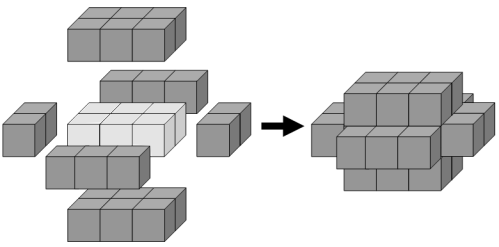
\includegraphics[width=70mm]{problems/101-200/meta/p126.png}};
    \end{tikzpicture}
\end{center}

If we then add a second layer to this solid it would require forty-six cubes to cover every visible face, the third layer would require seventy-eight cubes, and the fourth layer would require one-hundred and eighteen cubes to cover every visible face.

However, the first layer on a cuboid measuring $5 \times 1 \times 1$ also requires twenty-two cubes; similarly the first layer on cuboids measuring $5 \times 3 \times 1$, $7 \times 2 \times 1$, and $11 \times 1 \times 1$ all contain forty-six cubes.

We shall define $C(n)$ to represent the number of cuboids that contain $n$ cubes in one of its layers. So $C(22) = 2$, $C(46) = 4$, $C(78) = 5$, and $C(118) = 8$.

It turns out that $154$ is the least value of $n$ for which $C(n) = 10$.
\medskip

Find the least value of $n$ for which $C(n) = 1000$.


\section{abc-hits} \label{pb.0127}
%PB127

The radical of $n$, $rad(n)$, is the product of distinct prime factors of $n$. For example, $504 = 2^3 \times 3^2 \times 7$, so $rad(504) = 2 \times 3 \times 7 = 42$.

We shall define the triplet of positive integers $(a, b, c)$ to be an abc-hit if:

\begin{enumerate}
    \item $GCD(a, b) = GCD(a, c) = GCD(b, c) = 1$
    \item $a < b$
    \item $a + b = c$
    \item $rad(abc) < c$
\end{enumerate}
For example, (5, 27, 32) is an abc-hit, because:

\begin{enumerate}
    \item $GCD(5, 27) = GCD(5, 32) = GCD(27, 32) = 1$
    \item $5 < 27$
    \item $5 + 27 = 32$
    \item $rad(4320) = 30 < 32$
\end{enumerate}

It turns out that abc-hits are quite rare and there are only thirty-one abc-hits for $c < 1000$, with $\sum c = 12523$.

Find $\sum c$ for $c < 120000$.


\section{Hexagonal tile differences} \label{pb.0128}
%PB128

A hexagonal tile with number 1 is surrounded by a ring of six hexagonal tiles, starting at "12 o'clock" and numbering the tiles 2 to 7 in an anti-clockwise direction.

New rings are added in the same fashion, with the next rings being numbered 8 to 19, 20 to 37, 38 to 61, and so on. The diagram below shows the first three rings.

\begin{center}
    \begin{tikzpicture}
        \node[anchor=south west,inner sep=0] at (0,0) {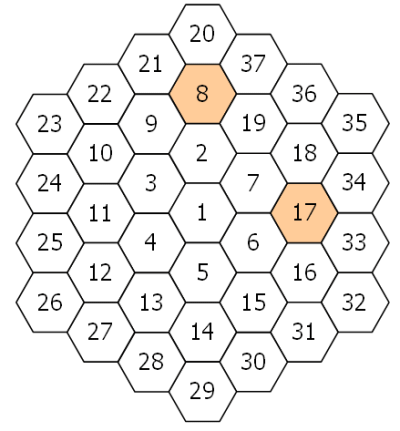
\includegraphics[width=70mm]{problems/101-200/meta/p128.png}};
    \end{tikzpicture}
\end{center}

By finding the difference between tile $n$ and each of its six neighbours we shall define $PD(n)$ to be the number of those differences which are prime.

For example, working clockwise around tile 8 the differences are $12, 29, 11, 6, 1$, and $13$. So $PD(8) = 3$.

In the same way, the differences around tile $17$ are $1, 17, 16, 1, 11,$ and $10$, hence $PD(17) = 2$.

It can be shown that the maximum value of $PD(n)$ is $3$.

If all of the tiles for which $PD(n) = 3$ are listed in ascending order to form a sequence, the $10^{\text{th}}$ tile would be $271$.

Find the $2000^{\text{th}}$ tile in this sequence.


\section{Repunit divisibility} \label{pb.0129}
%PB129

A number consisting entirely of ones is called a repunit. We shall define $R(k)$ to be a repunit of length $k$; for example, $R(6) = 111111$.

Given that $n$ is a positive integer and $GCD(n, 10) = 1$, it can be shown that there always exists a value, $k$, for which $R(k)$ is divisible by $n$, and let $A(n)$ be the least such value of $k$; for example, $A(7) = 6$ and $A(41) = 5$.

The least value of n for which A(n) first exceeds ten is 17.

Find the least value of n for which A(n) first exceeds one-million.


\section{Composites with prime repunit property} \label{pb.0130}
%PB130

A number consisting entirely of ones is called a repunit. We shall define $R(k)$ to be a repunit of length $k$; for example, $R(6) = 111111$.

Given that $n$ is a positive integer and $GCD(n, 10) = 1$, it can be shown that there always exists a value, $k$, for which R(k) is divisible by $n$, and let A(n) be the least such value of $k$; for example, $A(7) = 6$ and $A(41) = 5$.

You are given that for all primes, $p > 5$, that $p - 1$ is divisible by $A(p)$. For example, when $p = 41$, $A(41) = 5$, and $40$ is divisible by $5$.

However, there are rare composite values for which this is also true; the first five examples being $91, 259, 451, 481$, and $703$.

Find the sum of the first twenty-five composite values of $n$ for which
$GCD(n, 10) = 1$ and $n - 1$ is divisible by $A(n)$.


\section{Prime cube partnership} \label{pb.0131}
%PB131

There are some prime values, $p$, for which there exists a positive integer, $n$, such that the expression $n^3 + n^2p$ is a perfect cube.

For example, when $p = 19, 83 + 82 \times 19 = 123$.

What is perhaps most surprising is that for each prime with this property the value of $n$ is unique, and there are only four such primes below one-hundred.
\medskip

How many primes below one million have this remarkable property?


\section{Large repunit factors} \label{pb.0132}
%PB132

A number consisting entirely of ones is called a repunit. We shall define $R(k)$ to be a repunit of length $k$.

For example, $R(10) = 1111111111 = 11 \times 41 \times 271 \times 9091$, and the sum of these prime factors is $9414$.
\medskip

Find the sum of the first forty prime factors of $R(10^9)$.


\section{Repunit nonfactors} \label{pb.0133}
%PB133

A number consisting entirely of ones is called a repunit. We shall define $R(k)$ to be a repunit of length $k$; for example, $R(6) = 111111$.

Let us consider repunits of the form $R(10^n)$.

Although $R(10)$, $R(100)$, or $R(1000)$ are not divisible by $17, R(10000)$ is divisible by $17$. Yet there is no value of $n$ for which $R(10^n)$ will divide by $19$. In fact, it is remarkable that $11, 17, 41$, and $73$ are the only four primes below one-hundred that can be a factor of $R(10^n)$.
\medskip

Find the sum of all the primes below one-hundred thousand that will never be a factor of $R(10^n)$.


\section{Prime pair connection} \label{pb.0134}
%PB134


Consider the consecutive primes $p_1 = 19$ and $p_2 = 23$. It can be verified that $1219$ is the smallest number such that the last digits are formed by p1 whilst also being divisible by $p_2$.

In fact, with the exception of $p_1 = 3$ and $p_2 = 5$, for every pair of consecutive primes, $p_2 > p_1$, there exist values of $n$ for which the last digits are formed by $p_1$ and $n$ is divisible by $p_2$. Let $S$ be the smallest of these values of $n$.

Find $\sum S$ for every pair of consecutive primes with $5 \leqslant p_1 \leqslant 1000000$.


\section{Same differences} \label{pb.0135}
%PB135

Given the positive integers, $x, y$, and $z$, are consecutive terms of an arithmetic progression, the least value of the positive integer, $n$, for which the equation, $x^2 - y^2 - z^2 = n$, has exactly two solutions is $n = 27$:

$$34^2 - 27^2 - 20^2 = 12^2 - 9^2 - 6^2 = 27$$

It turns out that $n = 1155$ is the least value which has exactly ten solutions.
\medskip

How many values of $n$ less than one million have exactly ten distinct solutions?


\section{Singleton difference} \label{pb.0136}
%PB136

The positive integers, $x, y$, and $z$, are consecutive terms of an arithmetic progression. Given that $n$ is a positive integer, the equation, $x2 - y2 - z2 = n$, has exactly one solution when $n = 20$:

$$13^2 - 10^2 - 7^2 = 20$$

In fact there are twenty-five values of $n$ below one hundred for which the equation has a unique solution.
\medskip

How many values of $n$ less than fifty million have exactly one solution?



\section{Fibonacci golden nuggets} \label{pb.0137}
%PB137

Consider the infinite polynomial series $A_F(x) = xF_1 + x^2F_2 + x^3F_3 + \cdots$, where $F_k$ is the $k^{\text{th}}$ term in the Fibonacci sequence: $1, 1, 2, 3, 5, 8, ... $; that is, $F_k = F_{k-1} + F_{k-2}$, $F_1 = 1$ and $F_2 = 1$.
\medskip

For this problem we shall be interested in values of $x$ for which $A_F(x)$ is a positive integer.
\medskip

Surprisingly :

\begin{tabular}{rl}
    $A_F\left(\frac{1}{2}\right)$ & $= \left(\frac{1}{2}\right).1 + \left(\frac{1}{2}\right)^2.1 + \left(\frac{1}{2}\right)^3.2 + \left(\frac{1}{2}\right)^4.3 + \left(\frac{1}{2}\right)^5.5 + \cdots$\\
     & $= \frac{1}{2} + \frac{1}{4} + \frac{2}{8} + \frac{3}{16} + \frac{5}{32} + \cdots$\\
     & $= 2$\\
\end{tabular}
\medskip

The corresponding values of $x$ for the first five natural numbers are shown below.
\begin{center}
    \begin{tabular}{|l|c|}
        \hline
        $x$ & $A_F(x)$\\
        \hline
        $\sqrt{2}-1$ & $1$\\
        \hline
        $1/2$ & 2\\
        \hline
        $(\sqrt{13}-2)/3$ & $3$\\
        \hline
        $(\sqrt{89}-5)/8$ & $4$\\
        \hline
        $(\sqrt{34}-3)/5$ & $5$\\
        \hline
    \end{tabular}
\end{center}


We shall call $A_F(x)$ a golden nugget if $x$ is rational, because they become increasingly rarer; for example, the $10^{\text{th}}$ golden nugget is $74049690$.

Find the $15^{\text{th}}$ golden nugget.



\section{Special isosceles triangles} \label{pb.0138}
%PB138

Consider the isosceles triangle with base length, $b = 16$, and legs, $L = 17$.

\begin{center}
    \begin{tikzpicture}[scale=0.3]
        \draw[thick] (-8,0) -- (0,15) -- (8,0) -- cycle;
        \draw (0,0) -- (0,15);
        \draw[latex-latex] (-8,-0.5) -- (8,-0.5);
        \node[below] at (0,-0.5) {$b$};
        \node[left] at (0,7) {$h$};
        \node[left] at (-5,7) {$L$};
        \node[right] at (5,7) {$L$};
        
    \end{tikzpicture}
\end{center}

By using the Pythagorean theorem it can be seen that the height of the triangle, $h = \sqrt{(17^2 - 8^2)} = 15$, which is one less than the base length.

With $b = 272$ and $L = 305$, we get $h = 273$, which is one more than the base length, and this is the second smallest isosceles triangle with the property that $h = b \pm 1$.

Find $\sum L$ for the twelve smallest isosceles triangles for which $h = b \pm 1$ and $b, L$ are positive integers.



\section{Pythagorean tiles} \label{pb.0139}
%PB139

Let $(a, b, c)$ represent the three sides of a right angle triangle with integral length sides. It is possible to place four such triangles together to form a square with length $c$.

For example, $(3, 4, 5)$ triangles can be placed together to form a $5$ by $5$ square with a $1$ by $1$ hole in the middle and it can be seen that the $5$ by $5$ square can be tiled with twenty-five 1 by 1 squares.

\begin{center}
    \begin{tikzpicture}[scale=1]
        \draw(0,0) -- (0,5) -- (5,5) -- (5,0) -- cycle;
        \draw (0,1) -- (5,1)  (0,2) -- (5,2)  (0,3) -- (5,3)  (0,4) -- (5,4)  (1,0) -- (1,5)  (2,0) -- (2,5)  (3,0) -- (3,5)  (4,0) -- (4,5);
        
        \draw (-6,0) -- (-6,5) -- (-1,5) -- (-1,0) -- cycle;
    \end{tikzpicture}
\end{center}

However, if $(5, 12, 13)$ triangles were used then the hole would measure $7$ by $7$ and these could not be used to tile the $13$ by $13$ square.

Given that the perimeter of the right triangle is less than one-hundred million, how many Pythagorean triangles would allow such a tiling to take place?


\section{Modified Fibonacci golden nuggets} \label{pb.0140}
%PB140

Consider the infinite polynomial series $A_G(x) = xG_1 + x^2G_2 + x^3G_3 + \cdots,$ where Gk is the $k^{\text{th}}$ term of the second order recurrence relation $G_k = G_{k-1} + G_{k-2}$, $G_1 = 1$ and $G_2 = 4$; that is, $1, 4, 5, 9, 14, 23, ...$ .


For this problem we shall be concerned with values of $x$ for which $A_G(x)$ is a positive integer.

The corresponding values of $x$ for the first five natural numbers are shown below.

\begin{center}
    \begin{tabular}{|l|c|}
        \hline
        $x$ & $A_G(x)$\\
        \hline
        $(\sqrt{5}-1)/4$ & $1$\\
        \hline
        $2/5$ & $2$\\
        \hline
        $(\sqrt{22}-2)/6$ & $3$\\
        \hline
        $(\sqrt{137}-5)/14$ & $4$\\
        \hline
        $1/2$ & $5$\\
        \hline
    \end{tabular}
\end{center}

We shall call $A_G(x)$ a golden nugget if $x$ is rational, because they become increasingly rarer; for example, the $20^{\text{th}}$ golden nugget is 211345365.

Find the sum of the first thirty golden nuggets.


\section{Investigating progressive numbers, $n$, which are also square} \label{pb.0141}
%PB141

A positive integer, n, is divided by d and the quotient and remainder are q and r respectively. In addition d, q, and r are consecutive positive integer terms in a geometric sequence, but not necessarily in that order.

For example, 58 divided by 6 has quotient 9 and remainder 4. It can also be seen that 4, 6, 9 are consecutive terms in a geometric sequence (common ratio 3/2).
We will call such numbers, n, progressive.

Some progressive numbers, such as 9 and 10404 = 1022, happen to also be perfect squares.
The sum of all progressive perfect squares below one hundred thousand is 124657.

Find the sum of all progressive perfect squares below one trillion $(10^12)$.


\section{} \label{pb.0142}
%PB142


\section{} \label{pb.0143}
%PB143


\section{} \label{pb.0144}
%PB144


\section{} \label{pb.0145}
%PB145


\section{} \label{pb.0146}
%PB146


\section{} \label{pb.0147}
%PB147


\section{} \label{pb.0148}
%PB148


\section{} \label{pb.0149}
%PB149


\section{} \label{pb.0150}
%PB150



\setcounter{section}{150}
\section{} \label{pb.0151}
%PB151


\section{} \label{pb.0152}
%PB152


\section{} \label{pb.0153}
%PB153


\section{} \label{pb.0154}
%PB154


\section{} \label{pb.0155}
%PB155


\section{} \label{pb.0156}
%PB156


\section{} \label{pb.0157}
%PB157


\section{} \label{pb.0158}
%PB158


\section{} \label{pb.0159}
%PB159


\section{} \label{pb.0160}
%PB160


\section{} \label{pb.0161}
%PB161


\section{} \label{pb.0162}
%PB162


\section{} \label{pb.0163}
%PB163


\section{} \label{pb.0164}
%PB164


\section{} \label{pb.0165}
%PB165


\section{} \label{pb.0166}
%PB166


\section{} \label{pb.0167}
%PB167


\section{} \label{pb.0168}
%PB168


\section{} \label{pb.0169}
%PB169


\section{} \label{pb.0170}
%PB170


\section{} \label{pb.0171}
%PB171


\section{} \label{pb.0172}
%PB172


\section{} \label{pb.0173}
%PB173


\section{} \label{pb.0174}
%PB174


\section{} \label{pb.0175}
%PB175



%\setcounter{section}{175}
%\section{} \label{pb.0176}
%PB176


\section{} \label{pb.0177}
%PB177


\section{} \label{pb.0178}
%PB178


\section{} \label{pb.0179}
%PB179


\section{} \label{pb.0180}
%PB180


\section{} \label{pb.0181}
%PB181


\section{} \label{pb.0182}
%PB182


\section{} \label{pb.0183}
%PB183


\section{} \label{pb.0184}
%PB184


\section{} \label{pb.0185}
%PB185


\section{} \label{pb.0186}
%PB186


\section{} \label{pb.0187}
%PB187


\section{} \label{pb.0188}
%PB188


\section{} \label{pb.0189}
%PB189


\section{} \label{pb.0190}
%PB190


\section{} \label{pb.0191}
%PB191


\section{} \label{pb.0192}
%PB192


\section{} \label{pb.0193}
%PB193


\section{} \label{pb.0194}
%PB194


\section{} \label{pb.0195}
%PB195


\section{} \label{pb.0196}
%PB196


\section{} \label{pb.0197}
%PB197


\section{} \label{pb.0198}
%PB198


\section{} \label{pb.0199}
%PB199


\section{} \label{pb.0200}
%PB200




    %\include{problems_FR/201-300/pack_0201-0300}
    %\include{problems_FR/301-400/pack_0301-0400}
    %\include{problems_FR/401-500/pack_0401-0500}
    %\include{problems_FR/501-600/pack_0501-0600}
    %\include{problems_FR/601-700/pack_0601-0700}
    
\end{document}
